\chapter{MapReduce}

\section{Workflow}

Figure \ref{fig:MR-workflow} shows the adopted workflow\footnote{It is not the optimal one since the same query could be executed in less than four job. The idea is to structure the workflow this way so that few different MR algorithms can be applied (e.g. filtering, projection, summarization, join). }.

\begin{figure}[H]
	\centering
	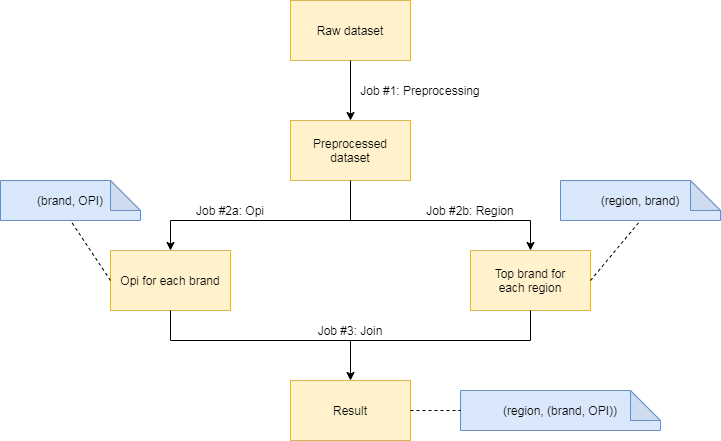
\includegraphics[scale=0.6]{images/2-mapreduce/MR-workflow.png}
	\caption{Adopted workflow for MR jobs.}
	\label{fig:MR-workflow}
\end{figure}

\section{Jobs}

\subsection{Job 1: Preprocessing}

The job executes all preprocessing operation needed to correctly use the dataset in next jobs. In particular, it fulfills the following goals:

\begin{itemize}

  \item \textbf{Cut out header}: the raw dataset is a csv file. The header must be eliminated.
  \item \textbf{Drop useless columns}.
  \item \textbf{Drop incomplete records}: record that have missing values on mandatory fields are simply dropped. 

Job execution and interfaces are described in figure \ref{fig:MR-job-1}.
 
Raw records are read and parsed into ``Car'', i.e. custom ``Writable'' objects, during map stage. 
Each car stores data about:
\begin{itemize}
 \item Region
 \item Price
 \item Brand
 \item Fuel
 \item Odometer
\end{itemize}

The map output is a pair where the key is the default key used by Hadoop when reading text files and the value is the car itself.

The reduce stage just replaces the default key with a ``NullableWritable'' so that the whole job output is a set of records yet.

\begin{figure}[H]
	\centering
	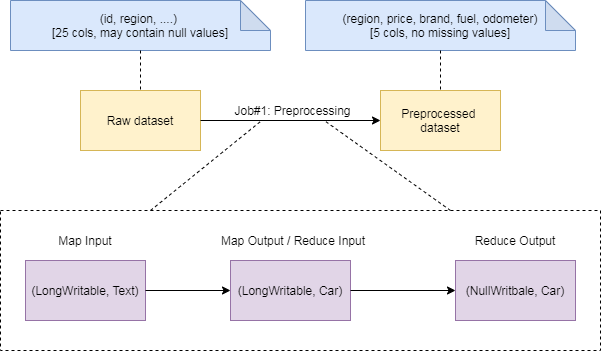
\includegraphics[scale=0.7]{images/2-mapreduce/MR-job-1.png}
	\caption{Description of ``job 1: preprocessing'' workflow and interfaces.}
	\label{fig:MR-job-1}
\end{figure}


%The dataset cardinality is reduced from 423858 to 231157.
%The dataset size is reduced from 1GB to 100MB.


\end{itemize}

\subsection{Job 2a: Opi}

The job executes the calculation of the OPI for each existing brand.

Job execution and interfaces are described in figure \ref{fig:MR-job-2a}.

The map stage input value is a car encoded as text. The key is the Hadoop default one for text files and its irrelevant. The mapper calculates the OPI for such car using price and odometer fields, and it gives as output a pair consisting of (brand, OPI).

The reduce stage just calculates the average value using single OPI values and reports it as output.
   
\begin{figure}[H]
	\centering
	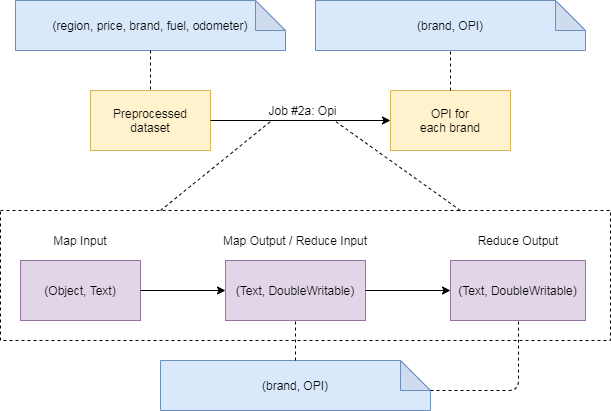
\includegraphics[scale=0.7]{images/2-mapreduce/MR-job-2a.png}
	\caption{Description of ``job 2a: opi'' workflow and interfaces.}
	\label{fig:MR-job-2a}
\end{figure}  

\subsection{Job 2b: Region}

The job goal is to find the most widespread brand in each region, namely the brand that has the most number of car on sale in a given region.

Job execution and interfaces are described in figure \ref{fig:MR-job-2b}.

The map stage input value is a car encoded as text. The key is the Hadoop default one for text files and its irrelevant. If the fuel type is correct, the mapper generates as output a pair (region, brand) so that reduce stage can operate per region basis.

The reducer, given a region, firstly calculates the cardinality for each brand by collecting the input pairs. Then, it calculates the maximum and gives it as output in the form of (region, brand).

\begin{figure}[H]
	\centering
	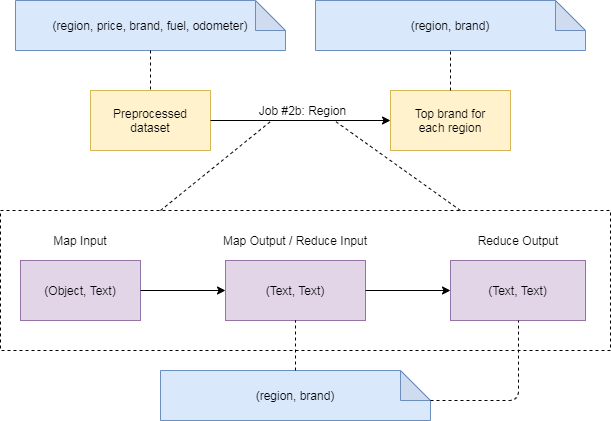
\includegraphics[scale=0.7]{images/2-mapreduce/MR-job-2b.png}
	\caption{Description of ``job 2b: region'' workflow and interfaces.}
	\label{fig:MR-job-2b}
\end{figure}  

\subsection{Job 3: Join}

Partial results of jobs 2a and 2b are combined into the final one. 

Job execution and interfaces are described in figure \ref{fig:MR-job-3}.

The map stage takes as input pairs structured as (Text, Text). The source of a given pair can be from job 2a output or from job 2b output. By examinating it, it is discovered the source and the pair is marked with a flag.
Since the join key will be the brand, the output of map stage is a pair (brand, (flag, region)), where flag and region are encapsulated into a ``JoinPair'' (a custom ``Writable'').

The reducer executes the standard join algorithm on input items and creates output pairs in the form (region, (brand, OPI)). 

\begin{figure}[H]
	\centering
	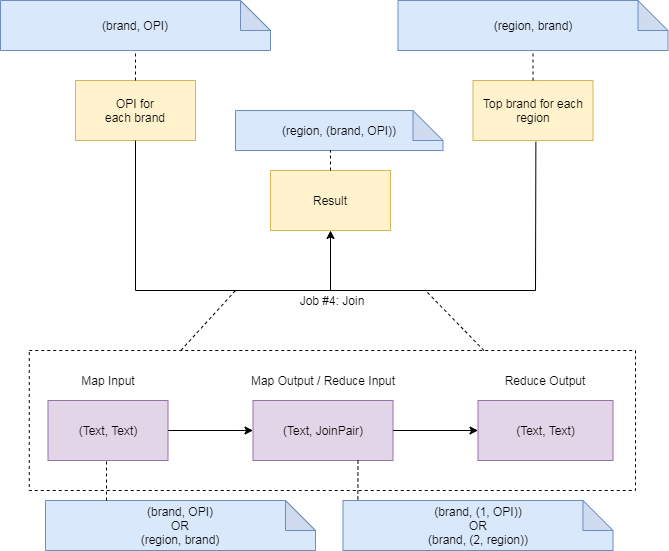
\includegraphics[scale=0.7]{images/2-mapreduce/MR-job-3.png}
	\caption{Description of ``job 3: join'' workflow and interfaces.}
	\label{fig:MR-job-3}
\end{figure}  


\section{Performance evaluation}

Performance are evaluated by varying the number of reducers and by enabling the use of combiners.

Each casuistry result is the average value upon 3 runs.

\begin{table}
  \centering
  \begin{tabular}{ |c c|c c c c c| } 
    \hline
    \multicolumn{2}{ |c| }{} & \multicolumn{5}{ c| }{Reducers} \\
    \multicolumn{2}{ |c| }{} & 1 & 2& 5& 10 & 100 \\
    \hline
    \multirow{2}{4em}{Combiner} 
    & No  & 223 & 162 & 168 & 216 & 1400 \\      
    & Yes &     &     &     &     &      \\ 
    \hline
  \end{tabular}
  \caption{Performance results expressed as elapsed time in seconds.}
\end{table}